% PARTIE 1 - PRESENTATION %%%%%%%%%%%
% CHAPITRE 2 %%%%%%%%%%%%%%%%%%%%%%%%
%%%%%%%%%%%%%%%%%%%%%%%%%%%%%%%%%%%%%
Ce deuxième chapitre explore le cadre numérique dans lequel s'est développé le projet Richelieu, en se concentrant particulièrement sur le volet RICH.DATA II. Il détaille les différentes étapes de traitement des données, depuis leur saisie par les équipes du projet jusqu'à leur mise en ligne sur une application Web destinée au public. En général, le traitement des données consiste en une série de processus visant à extraire de l'information et du savoir à partir de données brutes, avec pour objectif de les rendre intelligibles par l'ordinateur plutôt que directement lisibles par l'humain. Nous examinerons ainsi les spécificités de la chaîne de traitement des données du projet Richelieu.

%%%%%%%%%%%%%%%%%%%%%%%%%%%%%%%%%%%%%
% SECTION %%%%%%%%%%%%%%%%%%%%%%%%%%%
\section{Saisir la donnée : un enjeu pour l'interaction \\chercheur-ingénieur}
Dans le projet Richelieu, la saisie des données est réalisée à la fois par les chercheurs et les ingénieurs, en fonction des corpus. L'objectif est de construire un système d'information multidimensionnel comprenant les axes principaux du projet, pour rappel, l'iconographique, l'espace, le temps et le réseau. Cette partie abordera en détails les traitements effectués sur les principaux corpus, iconographie et cartographie, tandis que les corpus secondaires ne seront pas abordés.

\subsection{Annotation, description et structuration du corpus iconographique}
Une image est souvent accompagnée d'une légende précisant son titre, son auteur, et parfois sa date de création, la technique utilisée, ses dimensions, et son propriétaire. Au musée, cette légende prend la forme d'un cartel où le numéro d'inventaire peut être ajouté. Dans une notice bibliographique, qu'elle soit imprimée ou publiée en ligne, cette légende inclut également le lieu ou site Web de publication, l'éditeur ou le laboratoire de recherche associé, ainsi que la pagination. Ces références bibliographiques suivent diverses normes et styles, parmi lesquels les formats Harvard et Chicago sont les plus connus. Que ce soit sous forme de légende, de cartel, de notice ou de référence bibliographique, cette information décrit l'image, constituant ainsi la première couche enrichie d'informations. En somme, c'est une donnée sur la donnée et c'est ce qu'on nomme une métadonnée. Dans notre cas, il s'agit de métadonnées descriptives et structurelles, mais il en existe une grande variété (administratives, contextuelles, techniques, statiques, évolutives, externes aux contenu, etc.). Le volume des métadonnées est proportionnel à l'ampleur du corpus réuni, et il est donc particulièrement conséquent pour le projet Richelieu car les dimensions d'études sont plurielles. Il est donc pertinent de se demander : quelles sont les métadonnées du projet ? Soit, comment le corpus iconographique devient une donnée computationnelle et comment est-elle structurée dans ce système d'information ?

\subsubsection{Méthodologie appliquée}
Les données sont saisies \enquote{manuellement}, sans extraction automatique des métadonnées. Les chercheurs remplissent minutieusement les fichiers au format xls, un format propriétaire de Microsoft Excel, en complétant case par case, ligne par ligne et colonne par colonne. Ces tableurs, hébergés en ligne sur le serveur de l'\acrshort{inha}, permettent une complétion simultanée par plusieurs chercheurs. Initialement, chaque zone géographique du quartier — Vivienne, Bourse, \acrlong{bdf}, Richelieu — disposait de son propre tableur. Dans chacun des tableurs, on retrouve un onglet, ou feuille, par institution, un onglet consacré aux lieux et un onglet documentant l'évolution des différentes adresses par lieu car les numéros de rue peuvent changer avec les modifications parcellaires. Les colonnes des tableurs sont composé de plusieurs champs intitulés comme suit :  \enquote{Institution}, \enquote{\textcolor{blue}{Identifiant interne}}, \enquote{Manifest IIIF}, \enquote{IIIF Folio}, \enquote{\acrshort{url}}, \enquote{Titre}, \enquote{Auteur 1}, \enquote{Auteur 2}, \enquote{Editeur}, \enquote{Date Institution}, \enquote{\textcolor{red}{{Date corrigée}}}, \enquote{Technique}, \enquote{N° d'inventaire}, \enquote{Corpus}, \enquote{\textcolor{red}{Description iconographique}},\enquote{Marques, inscriptions, poinçons}, \enquote{\textcolor{red}{Commentaire historique}}, \enquote{\textcolor{blue}{Thème(s)}}, \enquote{\textcolor{blue}{Entité nommée}}, {\enquote{\textcolor{blue}{Id localisation}}}, \enquote{\textcolor{red}{Note interne}}, \enquote{Document produit imprimé ou vendu dans le quartier}, \enquote{Représente la ville ou les marchandises}\footnote{La casse est respectée dans la transcription des intitulés de colonnes.} -- totalisant 24 niveaux d’information distincts pour chaque document iconographique. Ce qui représente 96 000 métadonnées descriptives rien que pour le corpus iconographique, pour rappel, constitué de 4000 documents. 

Les métadonnées ayant fait l'objet de recherches supplémentaires par les équipes sont indiquées en \textcolor{red}{rouge}. Il s'agit d'annotations et de descriptions absentes des données brutes. En \textcolor{blue}{bleu}, sont mises en évidence les métadonnées structurelles, qui organisent l'objet documentaire selon la logique du système d'information du projet Richelieu. Par exemple, \enquote{Id localisation} relie chaque iconographie à une adresse ou à des repères spatiaux, permettant ainsi de géolocaliser les éléments représentés, que ce soit des immeubles, des points de vue, ou des lieux d'événements. Par exemple, RV2 désigne le 2, rue Vivienne, RVA15 le 15, rue de Valois, GC26 le 26, de la galerie Colbert, et RR65 le 65, rue Richelieu. Les adresses évoluent toutefois au fil du temps : par exemple, l'actuel 2, rue Vivienne était répertorié comme 2 et 4, rue Vivienne selon l’Atlas Vasserot (1810-1836), puis comme 2 et 2bis, rue Vivienne dans les atlas de 1860 à 1900. L'une des tâches principales des chercheurs est de reconstituer cette évolution. Par ailleurs, la métadonnée \enquote{Date corrigée} permet d'élargir la perspective temporelle du projet, tandis que \enquote{Thème(s)} et \enquote{Entité nommée} multiplient les accès à l'information.

% Le numéro d'inventaire dont nous avons cité en introduction de ce chapitre est plus exactement à considérer comme une métadonnée structurelle : il classifie l'œuvre selon un ordre ou une hiérarchie. Par exemple, le numéro d'inventaire \href{https://www.navigart.fr/picassoparis/artwork/pablo-picasso-autoportrait-160000000000541?page=1&filters=query%3AMP4}{MP4} signifie qu'il s'agit de la quatrième œuvre inventoriée lors de la succession Picasso pour la constitution du Musée national Picasso-Paris (MnPP). Tandis que le numéro d'inventaire \href{https://www.navigart.fr/picassoparis/artwork/pablo-picasso-portrait-d-olga-160000000001246?page=3&filters=tree_domain_all%3ADessin,,year%3A1921__1933}{MP1990-70} est la 70eme œuvre inventoriée en 1990 lors de la dation de Jacqueline Picasso pour le MnPP. Le projet Richelieu a également inventorier chaque document de son corpus : un identifiant unique lui est décerné. 

\subsubsection{Méthodologie recommandée}
Cependant, il est recommandé de contraindre la saisie des données par des règles, notamment pour assurer leur qualité. Laisser libre l'écriture avec majuscules, minuscules, espaces, signes de ponctuation, abréviations ou fautes de frappe augmente le risque d'erreur au lieu de le réduire. Comment garantir l'homogénéité et la qualité pour un volume important des données sans un cadre rigoureux ? L'outil utilisé dans le projet, Excel, propose un système de validation des données qui permet de définir divers critères, comme l'utilisation de masques de saisie pour restreindre les entrées. Il existe de nombreuses bonnes pratiques pour la saisie et la validation des données brutes, mais leur application dépend encore du contexte.

\subsubsection{Difficultés contextuelles}
En effet, ces contraintes deviennent difficiles à appliquer lorsque l'ingénieur intervient après qu'un premier travail de fouille, d'annotation, et de description des données ait été réalisé par les chercheurs, autrement dit par les équipes se succédant. De plus, le corpus se construit simultanément à sa description et à sa saisie. Le dépouillement d'un fonds, puis d'un autre, révèle des métadonnées descriptives intéressantes qui peuvent être absentes dans les collections déjà décrites. Une institution peut indiquer les multiples auteurs d'une œuvre alors qu'une institution se limitera à l'auteur principal. Ainsi, les métadonnées peuvent être enrichies par une collection, mais aussi entraîner un appauvrissement des informations pour une autre.

\subsubsection{Le rôle des standards et normes (ontologies, index, thésaurus)}
Pour surmonter certaines difficultés rencontrées lors de la saisie, on pourrait se demander : est-il possible d'extraire automatiquement les métadonnées à partir des bibliothèques numérisées ? Peut-on appliquer des normes et standards numériques dans le cadre du projet Richelieu pour faciliter la saisie ? L'extraction automatique n'est pas toujours à privilégier en raison de la diversité des structures de données utilisées par les bibliothèques et catalogues du musées numérisés. Ce constat s'explique par le fait que les institutions ne structurent pas leurs données de manière uniforme, même lorsqu'il existe des standards et des normes. Les ontologies, thésaurus, et index jouent un rôle structurant en fournissant des cadres normalisés pour harmoniser les données. Ces outils facilitent la recherche, l'interopérabilité, et l'exploitation des informations. Par exemple, il est recommandé aux institutions patrimoniales relevant des Musées de France de suivre les règles de l'export Joconde\footcite{MINISTEREDELACULTUREJoconde2024}. Pourtant, l'application de ces normes n'est pas obligatoire, et certaines institutions les adaptent tandis que d'autres ne les utilisent pas du tout tels que certains musées réunis sous l'établissement Paris Musées. En conséquence, les métadonnées descriptives varient considérablement d'une institution à l'autre, rendant l'harmonisation et l'extraction automatique plus difficile et questionnant la pérennité des données non standardisées. Enfin, malgré sa nature fastidieuse, la saisie manuelle reste une étape nécessaire voire indispensable pour garantir un contrôle qualité. Adopter des normes et standards dépend donc de la compatibilité avec les systèmes existants et des ressources (humaines et techniques) disponibles. Surtout, l'extraction est utile quand le corpus est bien identifié à l'inverse de celui du projet Richelieu qui l'a constitué au fur-et-à-mesure de la recherche. De plus, dans certains projets, notamment ceux ayant un objet central spécifique et un délai restreint, comme c'est le cas du projet Richelieu, il semble plus efficace de créer une grammaire de structuration des données sur-mesure plutôt que de tenter d'appliquer des standards externes. 


\subsubsection{Les formats d'entrée}
La saisie du corpus iconographique n'adhère pas à une norme standardisée de description des métadonnées. Toutefois, cette étape permet à l'ingénieur de produire un document au format conventionnel pour le traitement, tel que le \acrshort{csv}. Faisons remarquer que le corpus iconographique ne se compose pas de fichiers d'images tels que \acrshort{png}, \acrshort{jpg}, \acrshort{tiff} ou \acrshort{svg}. Au lieu de cela, il s'agit principalement d'\acrshort{url} (\textit{Uniform Resource Locator}), qui sont considérées comme des métadonnées à part entière. Ces \acrshort{url}, suivant le protocole \acrshort{iiif} (\textit{International Image Interoperability Framework}), offrent des avantages spécifiques, de volume et d'intéropérabilité des données sur le Web, que nous aborderons plus tard (voir le chapitre \ref{section:intero}). 

%%%%%%%%%%%%%%%%%%%%%%%%%%%%%%%%%%%%%
\subsection{Géoréférencement historique du corpus cartographique}
La numérisation des données cartographiques s'effectue par l'ingénieur en étroite collaboration avec l'équipe de chercheurs pour saisir et traiter ces informations. 

Pour rappel, une carte est une représentation à échelle réduite de la surface terrestre, et dans le cas du quartier Richelieu, cette réduction est particulièrement importante. Les cartes sont souvent accompagnées d'un graticule, une grille de lignes représentant un système de coordonnées géographiques. Pour se localiser sur une carte, on utilise un système de coordonnées composé d'un ensemble de repères constitués de points et lignes imaginaires : les pôles Nord et Sud, l'Équateur et ses parallèles alors croisés perpendiculairement par les méridiens. Une position géographique est le point d'intersection de deux de ces lignes, correspondant respectivement à la latitude (x) et à la longitude (y). L'une est déterminée par rapport à un méridien et l'autre par rapport à un parallèle. Parfois, une troisième dimension, l'altitude (z), est également considérée, elle est calculée vis-à-vis du niveau moyen de la mer. Aujourd'hui, la géolocalisation ou géopositionnement est  rapidement calculé par divers systèmes de navigation comme le \acrshort{gps} (états-unien), Glonass (russe), Galileo (européen), et Beidou (chinois). Dans le contexte de la numérisation de cartes et plans, les outils que manipule l'équipe, tel que \acrshort{qgis}, se base sur le \acrshort{gps} pour intégrer les données géographiques dans un plan en \acrshort{2d} qui applique une projection géodésique\footcite{GEOCONFLUENCESProjection2022} en Lambert 93. C'est sur cette base informatisée que le géoréférencement historique peut être effectué.


\subsubsection{\textit{Ti esti} le géoréférencement ... historique ?}
Le géoréférencement\footcite{GEOCONFLUENCESGeoreferencement2024} est un principe fondamental de la cartographie assistée par ordinateur (\acrshort{cao}). Il consiste à déterminer la position dans l'espace d'un objet en utilisant les données d'un système de coordonnées. L'objet n'a pas de coordonnées connues et le système de coordonnées permet de lui en donner. En l'occurrence, un plan historique de la ville de Paris est dépourvu de coordonnées informatiques. Si on le place sur une carte contemporaine numérisée, il se peut que tel mur de tel édifice patrimonial ne coïncide pas avec le même mur sur la carte contemporaine. Pour assurer une cohérence, on créé des points de contrôle, aussi appelées géoréférences, qui sont l'équivalent des éléments géographiques représentés sur les plans. Cette technique permet d'ajuster la carte à une projection choisie ou de changer d'échelle, ce qui est une opération courante dans le \acrlong{sig} (SIG)\footcite{BERNIERconcepts2014} dans lequel l'objet, la carte est un fichier raster (une image composée de pixels) et les coordonnées sont des objets vectoriels (des points, lignes, polylignes, polygones représentant les objets physiques). 

Mais qu'est-ce qu'une géoréférence historique, également appelée référentiel historique ? Aujourd'hui, la dimension géographique est de plus en plus intégrée dans les recherches en histoire, archéologie, et histoire de l'art, via la cartographie des territoires étudiés\footcite{ZOHARGeographic2022, TIMARWeb2024}. Le partage entre les communautés de chercheurs des éléments structurants l’espace géographique à différentes époques de temps, permet de gagner un temps précieux et est devenu une pratique courante. Ces éléments communs sont ce que l'on appelle un \enquote{référentiel géohistorique}. C’est l’un des objectifs majeurs du \acrshort{cstptm} que de constituer ces références géographiques et historiques afin d'en faciliter l’accès et l’usage. C’est en ce sens qu’un travail important a été engagé par le \acrshort{cstptm} sur le plan 1900 de Paris qu'exploite le projet Richelieu.

\subsubsection{Outils et méthodes}\label{par:méthodes}
Dans le cadre du projet Richelieu, l'équipe utilise principalement la méthode de géoréférencement par points de contrôle, une technique manuelle qui demande une grande précision. Cette méthode est appliquée aussi bien dans \acrshort{qgis} que dans l'outil \acrshort{galligeo}. 

\acrshort{qgis}, un logiciel libre de \acrshort{sig}, permet de créer des cartes géographiques et de gérer des données spatiales basées sur un modèle d'information géographique constitué de couches provenant de sources diverses. \acrshort{qgis} prend en charge les formats standardisés pour l'information géographique, y compris les fichiers raster\footnote{Un raster est une grille appelée matrice composée de cellules organisées en ligne et en colonne. Chaque celllule est un pixel unique. Chaque pixel a des valeurs, de couleurs par exemple. L'association de l'ensemble des pixels crée une image. Plus communément, si on zoom sur cette image et qu'elle est pixelisée car la netteté se dégrade, c'est alors un raster.} et vectoriels\footnote{Un fichier vectoriel n'est pas composé de pixels mais contient des attributs (les informations descriptives qui lui sont associées) et une géométrie (sa forme créée de point, ligne et polygone)}. En résumé, un fichier raster est une image composée de pixels, tandis qu'un fichier vectoriel représente des objets physiques par des points, lignes, et polygones alors calculables par l'ordinateur. C'est pourquoi les données raster, bien que plus complexes à analyser, sont souvent utilisées comme fonds de cartes, sur lesquelles des données vectorielles sont superposées. C'est une image que l'on vient enrichir d'informations. Cependant, bien que \acrshort{qgis} dispose d'un module intégré pour le géoréférencement, appliquer cette technique à des plans historiques peut s'avérer complexe en raison de l'absence de graticules nécessaires pour un géoréférencement absolu, rendant le géoréférencement historique relatif.

Le projet Richelieu enrichit les fonds de cartes historiques en intégrant des informations sur l'évolution du tissu urbain, informatisées sous forme de polygones représentant l'emprise au sol des bâtiments. Chaque polygone est associé à des coordonnées géographiques (x et y) et une clé d'identification, et le travail finalisé est sauvegardé au format \textit{shapefile}. Les fichiers raster utilisés initialement sont généralement au format \acrshort{geotif}, robuste et polyvalent. Pour créer ces fichiers, l'équipe utilise la plateforme \acrshort{galligeo}, développée par Eric Mermet du Pôle géomatique\footcite{ALPAGEGlossaire2024} de l’\acrshort{ehess} (membre fondateur du \acrshort{cstptm}). \acrshort{galligeo} applique des méthodes similaires de géoréférencement par points de contrôle pour des cartes anciennes disponibles sur Gallica, la bibliothèque numérique de la \acrshort{bnf}. Cet outil en ligne récupère l’\acrshort{url} de la carte-image sur Gallica, puis l'utilisateur identifie des points homologues sur l'image et sur des cartes contemporaines déjà géoréférencées. Ce processus se déroule en flux de données, sans téléchargement, permettant aux utilisateurs de constituer une collection de cartes géoréférencées accessibles en ligne via un \acrshort{sig}. Ce flux de données, déjà utilisé dans le projet \acrshort{anr} ALEGORIA\footcite{ENSG-GEOMATIQUEIGNProjet2022} pour des fonds iconographiques, est particulièrement innovant dans le contexte des cartes historiques.

Une autre méthode utilisée pour le géoréférencement est la méthode dite \enquote{régressive}. Celle-ci repose sur un plan vectoriel actuel des îlots, du réseau des voies et des adresses. Le processus commence par l'identification des éléments qui n'ont pas changé depuis une date précise, comme 1900. Ensuite, des corrections mineures sont apportées aux objets ayant subi de légères modifications, et ceux qui ont disparu ou ont été profondément transformés sont reconstitués. Cette approche réduit considérablement le travail de saisie, permettant de gagner un temps précieux, et facilite la superposition des cartes anciennes successives jusqu'à aujourd'hui, en identifiant les changements par rapport aux éléments constants. Grâce à cette méthode, divers procédés ont été développés pour gérer les \enquote{créations, disparitions et transformations}, permettant ainsi aux acteurs du \acrshort{cstptm} de reconstituer environ 5 000 îlots de 1900 à partir des quelque 7 500 îlots actuels, 3 900 voies de 1900 à partir des 6 000 actuelles, 17 000 tronçons de voies de 1900 à partir des 36 000 actuels, et enfin 118 700 points d’adresse de 1900 à partir des 150 000 actuels sur tout Paris. 

L'alignement des cartes anciennes avec la topographie actuelle nécessite l'utilisation de divers outils et méthodes développés par un large réseau, mettant en lumière l'importance de l'interdisciplinarité. La collaboration étroite entre chercheurs et ingénieurs exige une adaptation mutuelle, alliant les contraintes de l’ingénierie numérique et documentaire aux exigences scientifiques de l’histoire du tissu urbain, pour atteindre un objectif commun : la spatialisation des données historiques.

% \subsection{Le corpus textuel par extraction}
% La donnée du corpus textuel est extraite par océrisation. Ces documents écrits possèdent la même structure : 3 colonnes, dont chacune est censé recenser la même information. Chacune des colonne représente un segment à océriser, soit une image unique par colonne. L'outil de segementation des images utilisé est dhSegment \note[MC]{Mettre un lien vers cet outil, ou le décrire rapidement}. Sur un modèle de 90 pages segmentées à la main, 27 000 pages ont ainsi pu être segmentées. Concernant l'OCR, l'outil de Google Cloud Vision a été privilégié car il semblerait que les chiffres soient plus facilement lisibles \note[MC]{Dans l'idéal, il faudrait le justifier avec certitude (mais cela est sûrement compliqué dans ton cas si tu n'as pas participé aux études sur GCV): un lien vers une étude, vers une annexe, ou bien un tableau des comparaisons qui ont amené à ce choix.}. Puis, un premier alignement de ces deux jeux de données a été effectué. Mais, sur les 4 millions de lignes, seules un très faible pourcentage de ce traitement obtient un bon score de lisibilité. La troisième colonne n'enregistre pas les données de façon uniforme. C'est pourquoi seules 1000 lignes constituent le corpus textuel du projet Richelieu une fois traité. 

% %%%%%%%%%%%%%%%%%%%%%%%%%%%%%%%%%%%%%
% \subsection{Les corpus secondaires}
% \subsubsection{Le corpus photogrammétrique}
% Une spatialisation des points de vue depuis lesquels la Place de la Bourse est représentée dans notre corpus iconographie => cf multidimensionnalité du projet de F. Clavaud. Un exemple d'ontologie descriptives : RICO et les données géographiques. 
% \note[MH]{Intégrer screen des différentes prises de point de vue des photos}

\subsubsection{Conclusion}
La saisie de la donnée est un processus particulièrement long pour les équipes du projet Richelieu qui a su faire appel à divers outils et méthodes reflétant les ambitions d'exhaustivité du système d'information géolocalisé. Mais elle ne constitue que la première étape de la chaîne de traitement, la modélisation de la donnée étant la suivante.

%%%%%%%%%%%%%%%%%%%%%%%%%%%%%%%%%%%%%
% SECTION %%%%%%%%%%%%%%%%%%%%%%%%%%%
\section{Modéliser la donnée : le lieu comme objet central}
La modélisation des données est une étape essentielle pour l'intégration en base de données. Ce processus consiste à créer une représentation d'un domaine de connaissances, ou d'un objet réel, sous la forme d'une structure de données dont les relations sont clairement définies pour ensuite être étudiées, manipulées et comprises\footcite{FLANDERSShape2018}. Il s'agit de formaliser la logique du système pour identifier les éléments constitutifs, ainsi que leurs similitudes et différences. Cette étape permet également de structurer les enjeux de recherche du projet et d'y répondre par une modélisation qui envisage les corpus sous un angle commun et précis\footcite{SOUTOUModelisation2017}. Présenter et maîtriser les subtilités du modèle de données est une étape nécessaire pour préparer leur exposition sur une application. Dans le cadre du projet Richelieu, la question clé est : comment relier les différents corpus qui le composent ? Quelles sont leurs relations, leurs points communs et leurs différences ? Les exigences spatiales des données documentaires ont fortement influencé la réflexion et la définition du modèle de données du projet. Il est important de noter que plusieurs niveaux de modélisations informatiques existent : conceptuel, logique et physique - parmi lesquelles nous aborderons la modélisation conceptuelle qui présente les entités, les types et les relations définies, et, la modélisation physique pour son implémentation en SQl. 

\subsection{Le modèle conceptuel : le lieu comme entité centrale.}

Le modèle conceptuel de données consiste à représenter visuellement et de façon simplifiée la structure des données d'un système d'information. Pour ce faire, et, dans le cadre du projet Richelieu, on se demande comment modéliser la notion d'espace entre les différents corpus ? Pour y parvenir, le projet a dû surmonter plusieurs contraintes logiques, explorant diverses modélisations avant de converger vers la notion de lieu\footcite{KERVEGANmarque2023}. Par exemple, l'adresse a été envisagée comme entité centrale, mais cela ne permettait pas de représenter l'évolution du tissu urbain, comme dans le cas du 2, rue Vivienne, évoqué précédemment. Une autre approche consistait à utiliser les coordonnées géographiques (x, y) comme point de référence, une méthode couramment appliquée dans des projets similaires. Cependant, ce modèle présentait des problèmes logiques liés à l'échelle réduite du quartier : où placer précisément le point sur un édifice — sur la façade, à l'arrière, dans la cour, etc. ? De plus, cette solution ne répondait pas aux enjeux scientifiques du projet, qui se concentrent sur la réalité bâtie.

Ainsi, la modélisation par le lieu s'est révélée être une approche plus appropriée compte tenu de la masse de données à traiter :
\begin{displayquote}{\enquote{La chaîne de traitement mise au point pour le projet est définie autour d'un objet central : le lieu. Cette entité, définie dans le temps et dans l’espace, et représentée par des ressources iconographiques et cartographiques. Elle est également un espace de vie, habité et pratiqué. Le lieu est donc capable de croiser les composantes spatiales, architecturales, socio-économiques, historiques et culturelles du quartier. C’est un objet qui permet de faire dialoguer les différents corpus et d’étudier la spatialité du quartier ; c’est donc autour de lui que la chaîne de traitement a été développée.}}\footcite{PROJETFondation2023} 
\end{displayquote}

Le lieu, en tant qu'entité centrale, permet de décloisonner les corpus spécialisés et devient le socle commun pour un ensemble d'informations, jouant un rôle clé dans les opérations de géoréférencement. 

\begin{figure}
    \centering
    \includegraphics[width=1\linewidth]{images/modèle_conceptuel2.png}
    \caption{Modèle conceptuel du projet Richelieu, Paul Kervegan, 2023.}
    \label{fig:enter-label}
\end{figure}

\subsection{Le modèle physique de la base de données relationnelle.}\label{sous-section:modele-bddr}
La modélisation physique est une étape capitale qui précède l'implémentation des données dans un système de gestion de base de données. Pour le projet Richelieu, cela se traduit par l'utilisation d'une base de données relationnelle (\acrshort{bddr}), où les données sont structurées en tables (similaires à des tableurs), composées de champs (équivalents aux intitulés de colonnes). Ces tables sont interconnectées par des relations, toujours établies via des clés primaires et étrangères. Une clé étrangère dans une \acrshort{bddr} est un champ qui établit un lien entre deux tables en faisant référence à la clé primaire d'une autre table. Elle garantit l'intégrité référentielle car elle s'assure que la valeur existe dans la table correspondante. Une \acrshort{bddr} permet de réaliser des requêtes complexes pour manipuler et interroger les données de manière efficace. Le modèle physique du projet Richelieu est d'une complexité relative, comme en témoigne la représentation graphique \ref{fig:modele-physique-bdd}.
\begin{figure}
    \centering
    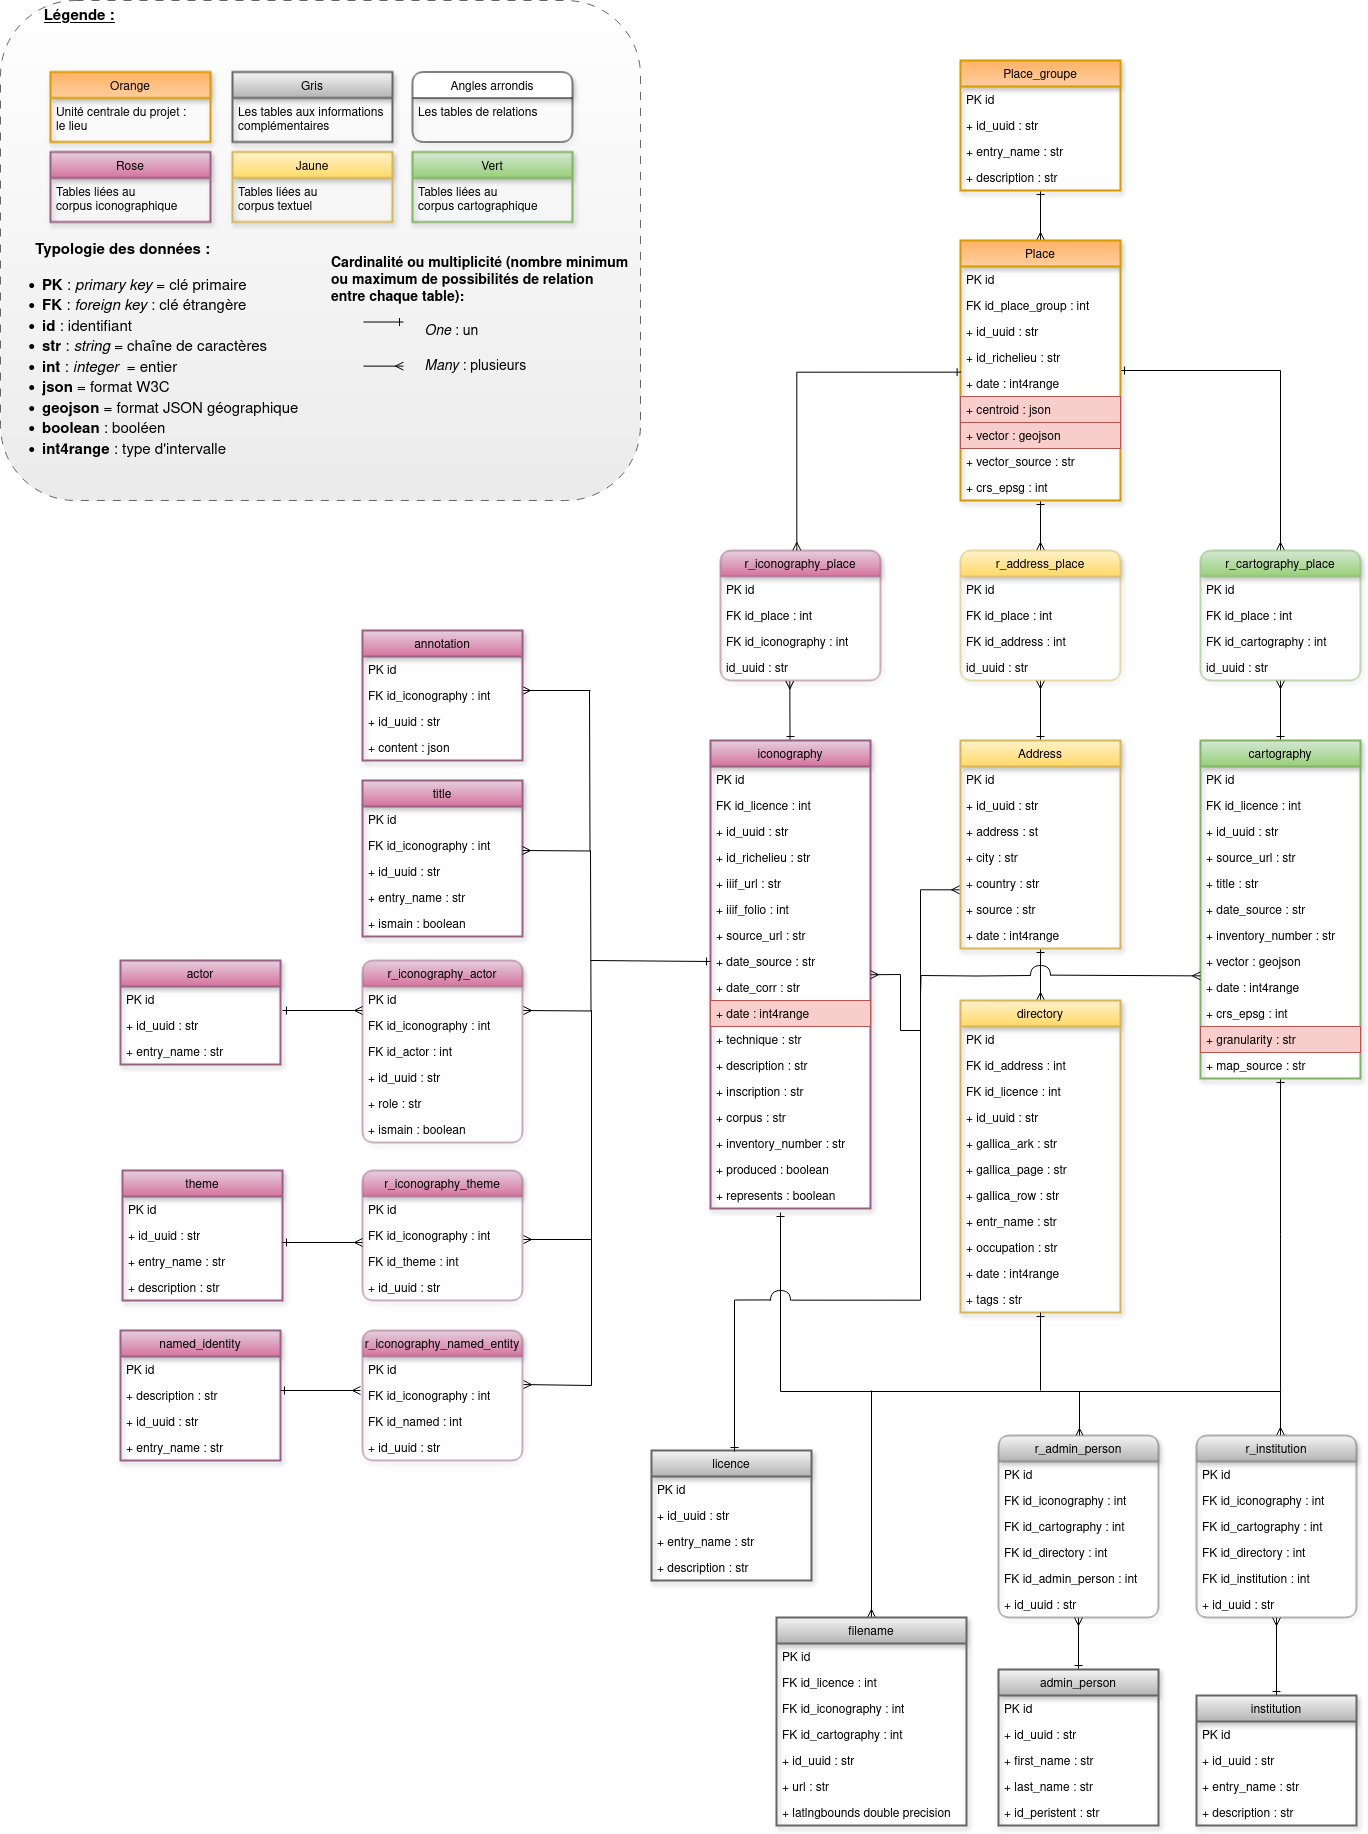
\includegraphics[width=1\linewidth]{images/modele-physique-bddr.drawio.png}
    \caption{Modèle physique des données du projet Richelieu, \mhd.}
    \label{fig:modele-physique-bdd}
\end{figure}

Examinons la structure du modèle dans ses grandes lignes. Ce modèle est organisé en plusieurs entités principales, chacune représentant une table dans la base de données. Au total, le modèle comprend 23 tables, regroupées par catégories fonctionnelles et différenciées par des couleurs spécifiques (par exemple, les tables en rose pour le corpus iconographique et celles en gris pour les informations administratives et descriptives reliées à l'ensemble des corpus). Chaque table possède une clé primaire (\acrshort{pk} : \textit{Primary Key}) qui permet d’identifier de manière unique chaque enregistrement. De nombreuses tables comportent également des clés étrangères (\acrshort{fk} : \textit{Foreign Key}) pour établir les relations entre elles, renforçant ainsi l'intégrité référentielle du modèle. Ainsi il y a 8 tables de relations, mais certaines relations se font en dehors de ces tables. Elles sont soit de type \enquote{un à plusieurs} soit \enquote{plusieurs à un}, comme l'indiquent les lignes connectant les tables. Elles sont essentielles pour maintenir la cohérence des données et permettre des jointures efficaces lors des requêtes. Par exemple, un lieu peut être associé à plusieurs documents iconographiques, cartographiques ou textuels, tandis qu'une licence spécifique peut s’appliquer à plusieurs sources documentaires.

Chaque table est constituée de divers champs, tels que des chaînes de caractères, des entiers ou des booléens, permettant de stocker une gamme variée d'informations comme des identifiants, des descriptions textuelles, des dates et des attributs spécifiques à la donnée spatiale. En plus des clés, le modèle comprend ainsi 85 attributs (les champs) qui structurent la diversité des informations. La définition des types de données est une étape importante pour assurer qu'elles respectent une qualité, une cohérence et une certaine forme d'intégrité. Le modèle présente également des associations complexes entre les tables, telles que celles entre \enquote{iconography} et \enquote{cartography}, soulignant l'interconnexion des données, comme le prévoyait le modèle conceptuel. On observe que la modélisation est pyramidale, avec toutes les informations convergeant via la table \enquote{place}, le lieu. En résumé, le modèle contient environ 30 000 lignes de données, sans compter les tables de relations, et plus de 104 000 données en incluant ces dernières. Le volume de données peut paraître moins conséquent que d'autres projets de recherche analogues, mais répartir ce volume à l'échelle du quartier est assez conséquent. On peut espérer que le modèle répond aux exigences pour la gestion d'un corpus de données riche, varié, complexe et multidimensionnel.

Nous avons mis en évidence en rouge certains enregistrements qui soulignent les particularités du modèle. Dans la table \enquote{cartography}, le champ \enquote{granularity} indique le niveau de détail ou de précision des données cartographiques. La granularité est classée en cinq catégories : \enquote{ensemble}, \enquote{aile}, \enquote{galerie}, \enquote{parcelle} et \enquote{point}, chacune correspondant à une échelle de représentation du quartier. Par exemple, le Palais Royal est étudié comme un ensemble architectural, mais ses différentes ailes (Beaujolais, Montpensier, Valois) et galeries (galerie de Bois devenue galerie d'Orléans) sont également détaillées. Cette granularité reflète la diversité de la réalité bâtie du quartier Richelieu.
Nous notons que la date est souvent enregistrée, mais avec plusieurs typologies attribuées. Dans la table \enquote{iconography}, un travail approfondi de datation des sources iconographiques a été réalisé par l'équipe de recherche. De nombreuses incohérences temporelles ont été constatées dans les notices des documents, conduisant à une correction manuelle et à la création d'une typologie spécifique. Lorsqu'une date précise est inconnue ou erronée, un intervalle de dates est utilisé plutôt qu'une date unique. Ce type de données permet de stocker des plages de dates dans une seule colonne de manière compacte, bien que le type \enquote{daterange} existe et aurait pu être une alternative.
Enfin, examinons les données de la table \enquote{place}, où les champs \enquote{centroid} et \enquote{vector} utilisent des structures de données incluant des informations géographiques, telles qu'un polygone qui a pour valeur des coordonnées géographiques (x,y). Le format \acrshort{geojson}, basé sur un système de \enquote{clé~:~valeur}, est particulièrement adapté pour stocker ces données complexes qui sont difficiles à représenter dans des colonnes traditionnelles\footcite{Definition2024}. Ce format est donc très utile pour les applications nécessitant des informations géospatiales, comme c'est le cas pour le projet Richelieu.

Ainsi, la granularité, les dates, les vecteurs et la richesse des données iconographiques correspondent aux dimensions que le projet souhaite modéliser : l'espace, le temps et l'iconographie. Cependant, la dimension du réseau semble être implicite dans le modèle, à moins qu'elle ne soit représentée par le nombre d'interconnexions présentes. Une analyse plus approfondie du contenu de la base de données permettra de clarifier cette question, ce qui sera exploré dans la prochaine partie.

En conclusion, il est évident que la modélisation constitue une étape fondamentale. Sans elle, la modularisation du lieu et l'identification de certains avantages n'auraient pas été possibles. Elle permet de décomposer la complexité en fragments plus simples, de diviser l'objet principal en objets secondaires pour une gestion autonome, tout en préservant les connexions nécessaires entre ces objets grâce au modèle de données relationnel.

%%%%%%%%%%%%%%%%%%%%%%%%%%%%%%%%%%%%%
% SECTION %%%%%%%%%%%%%%%%%%%%%%%%%%%
\section{Encoder pour stocker la donnée}
Définir la modélisation d'une base de données et les types à respecter ne suffit pas à la créer, il faut encore l'encoder afin de préparer son stockage dans un système de gestion de base de données. Cette étape est le cœur du traitement de la donnée, le \enquote{\textit{data cleaning}} (nettoyage des données) et le \enquote{\textit{data formatting}} (formatage des données) peuvent alors être effectué.

\subsection{\textit{Data Cleaning}}
Le nettoyage des données cherche à réduire le pourcentage d'erreurs suite à la saisie, réduire le \enquote{bruit} environnant les données. Cette étape a ainsi pour but d'assurer la qualité des données afin que celles-ci respectent les contraintes et règles définies, assurant aussi leur harmonisation. Cette étape est d'autant plus essentielle lorsque les données sont saisies manuellement. 

Dans le projet Richelieu, le nettoyage des données est une tâche considérable. Il faut d'abord s'assurer de nettoyer les tableurs en supprimant les en-têtes des colonnes et les colonnes vides à la fin des fichiers. Le nettoyage automatique, bien que précis, rencontre des difficultés pour corriger les fautes de frappe, gérer les valeurs manquantes, les doublons, et respecter la casse. Cela souligne l'importance de définir des règles strictes dès la saisie des données.

Cependant, l'équipe ingénieur-chercheur a trouvé des solutions pour surmonter certains problèmes de saisie : l'utilisation du \textit{pipe} ( | ) comme séparateur d'informations pour le traitement des entités nommées et des thèmes a permis de ne pas multiplier les colonnes à traiter, et d'éviter d'utiliser la virgule dont un traitement aurait été compliqué, au vue de son utilisation importante dans les autres cases du tableur. Le nettoyage principal se concentre sur la concaténation des fichiers pour qu'ils deviennent d'abord des jeux de données séparés puis formant un seul \textit{dataset}, tout en veillant à ce que les jointures entre les corpus soient possibles. Ensuite, des scripts Python sont développés pour associer les lignes aux fichiers image et vérifier qu'il n'y a pas de manque - auquel cas ils sont répertoriés dans un fichier annexe à destination des chercheurs qui doivent alors le compléter. Ce fichier est ensuite de nouveau traité pour être intégré au \textit{dataset} général. La conversion des fichiers (shapefiles en DataFrame ou \acrshort{geojson}, \acrshort{geotif} en \acrshort{png}) et l'harmonisation des coordonnées géographiques en EPSG:3857 / WGS84, le système de coordonnées cartésien utilisé par la bibliothèque JavaScript pour le développement de la carte, sont également effectuées. Nettoyer autant que possible garantit des données valides et facilite leur gestion par le système de base de données.

\subsection{\textit{Data Formatting}}
Après le nettoyage, vient l'étape du formatage des données, qui vise à rendre ces dernières compréhensibles pour l'ordinateur. Cela implique de standardiser les formats en adaptant les données aux exigences spécifiques de la base de données, et de s'assurer que les types de données sont corrects (par exemple, qu'un décimal n'est pas stocké comme un entier). Un travail particulier a été réalisé sur la normalisation des dates en utilisant le type \enquote{int4range}. La structuration du \textit{dataset} consiste ensuite à organiser les informations pour qu'elles correspondent à la structure des tables du modèle physique. Les quatre tables principales (iconographie, cartographie, textes, et lieux) sont traitées distinctement grâce à la librairie Pandas du langage de programmation Python.

Un aspect à relever de cette étape est la génération d'un système d'identification double pour chaque enregistrement de la donnée. D'une part, des clés primaires et étrangères sont créées pour chaque enregistrement. Même s'il ne s'agit pas d'identifiant à proprement parlé, les clés permettent toutefois d'identifier les données et sont essentielles pour le fonctionnement interne de la base de données, pour assurer la connexion entre les différentes tables. Les clés sont invisibles par le public. D'autre part, un \textit{Universal Unique Identifier} (\acrshort{uuid}) est généré pour chaque entrée. Ce code unique à 128 bits, composé de 36 caractères organisés en 5 groupes séparés par des tirets (8-4-4-4-12), garantit l'unicité de chaque enregistrement, même s'il est créé dans des environnements différents, à savoir dans plusieurs \textit{dataset}. Ce format est globalement unique, indépendant et sécurisé. Enfin, un autre système d'identification des documents est intégré au projet : \acrshort{ark}. L'\textit{Archival Resources Key} est un système persistant qui fournit des \acrshort{url} stables pour les ressources numériques, couramment utilisé dans les bibliothèques, archives et musées (dont la \acrshort{bnf} et d'où sont issus de nombreux documents du projet). Un identifiant \acrshort{ark} se compose d'une étiquette « \acrshort{ark}:/ », suivie d'un \acrshort{naan} (numéro d'autorité nommante) attribué par l'ARK Alliance, d'un nom d'identifiant alphanumérique associé à la ressource, et de qualificatifs. Ces qualificatifs incluent ceux de granularité, indiquant la position hiérarchique de la ressource, et de service, spécifiant la version ou le format de la ressource. Pour fonctionner, un identifiant \acrshort{ark} doit être associé à un résolveur utilisant un protocole d'accès (http:// ou https://) et le nom du serveur Web de l'autorité d'adressage (comme Gallica de la \acrshort{bnf}). Dans le cas de l'INHA, les \acrshort{uuid} ont tous le même préfixe \texttt{qr1} afin que le résolveur \acrshort{ark} de l'INHA puisse faire des redirections vers le site Richelieu. C'est un projet en cours de développement par le \acrshort{snr}. Ce système flexible s'adapte aux évolutions technologiques et aux modifications des ressources, assurant une accessibilité  pérenne\footcite{POCHONsysteme2021}. Enfin, rappelons que les identifiants \acrshort{ark} sont générés automatiquement, plus exactement ils sont moissonnés grâce à l'\acrshort{api} Gallica Rercherche, lors de cette étape de formatage des données. 

\begin{figure}
    \centering
    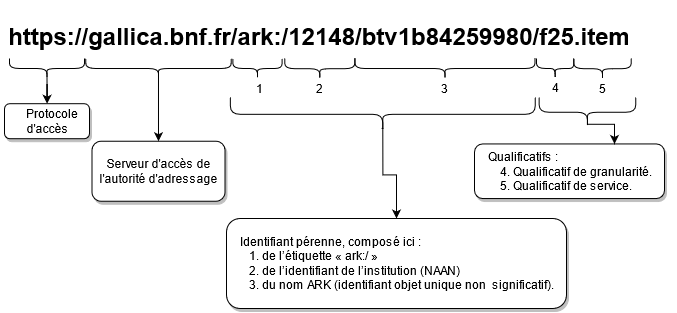
\includegraphics[width=1\linewidth]{images/schema-ark.png}
    \caption{Permalien disposant d'un identifiant \acrshort{ark},  Chloé Pochon, 2021.}
    \label{fig:ark}
\end{figure}

Vu le volume de données, l'étape de formatage semble considérable. En réalité, le travail effectué se concentre principalement sur le volume d'informations historiques car le volume des identifiants est créé automatiquement. Les identifiants sont plus que nécessaires car ils servent à retrouver et à distinguer les éléments de façon unique et sans ambiguïté. 

\subsection{Des données pour le Web}\label{sous-section:web}
Bien que le projet n'affiche pas la volonté de s'intégrer aux enjeux du Web sémantique, qui vise à rendre les données Web plus compréhensibles pour les machines à l'aide de standards et technologies pour décrire les relations entre les données, il intègre divers formats interopérables spécifiques au Web.

\textbf{\acrshort{iiif}} (\textit{International Image Interoperability Framework}) est un protocole d'échange destiné à standardiser la gestion des images numériques, allant de leur hébergement à leur visualisation\footcite{ROBINEAUComprendre2016}. \acrshort{iiif} facilite l'accès et la manipulation des images en utilisant un cadre commun d'interopérabilité, ce qui réduit les coûts de stockage et favorise une approche écologique des données. Les images, qu'elles soient de documents physiques alors numérisés ou des fichiers nativement numériques, sont accessibles directement depuis leur serveur d'origine, sans nécessiter de ré-hébergement ou de stockage local, même lorsqu'il s'agit de fichiers en très haute définition. Grâce aux \acrshort{api} \acrshort{iiif}, les institutions patrimoniales peuvent partager leurs images de manière standardisée\footcite{INHAbibliotheques2019} car \acrshort{iiif} définit des \acrshort{url} normées pour accéder à un fichier image. Les utilisateurs peuvent les manipuler via des requêtes \acrshort{url} (http(s) ://{domaine}/{identifiant}/{zone}/{taille}/{rotation}/{qualité}.{format})\footcite{FAUREstandard2022}, permettant des ajustements comme le cadrage, la rotation et le redimensionnement, tout en préservant les fichiers originaux sur le serveur d'origine. L'ensemble des documents numérisés et sélectionnés pour le projet Richelieu sont dotés d'\acrshort{url} \acrshort{iiif}. Ils seront donc accessibles en \acrshort{iiif} directement depuis l'application. Du point de vue de l'application, cela signifie que les images ne sont pas accessibles via un dossier d'images stockées sur un serveur \acrshort{inha}. Elles sont servies via un catalogue d'\acrshort{url}s aggrégeant des ressources stockées dans plusieurs bibliothèques numériques (\textit{\acrshort{iiif} Stores})\footcite{INHAbibliotheques2019}.

Le \textbf{\acrshort{json}} (\textit{JavaScript Object Notation}) est l'autre format léger utilisé en grande partie sur le projet. Facilement compréhensible pour un œil humain novice, il est utilisé pour structurer et échanger des données entre serveurs et clients, en particulier dans les applications Web. Sa structure simple repose sur des paires clé-valeur où les clés sont des chaînes de caractères et les valeurs peuvent être des chaînes, des nombres, des tableaux, des objets ou des booléens. Le \acrshort{geojson} est une norme de description de données spatiales au format \acrshort{json}. Il utilise les mêmes paires \enquote{clé~:~valeur} mais introduit des types géographiques tels que Point, Polygon, et MultiPolygon (pour ceux qui concernent le projet) pour encadrer les informations géographiques, avec des coordonnées exprimées en latitude et longitude selon le système WGS84, assurant une compatibilité étendue avec divers systèmes de cartographie. \acrshort{json} et \acrshort{geojson}, grâce à leur compatibilité avec de nombreux langages de programmation et leur adoption généralisée dans les \acrshort{api}, sont essentiels pour l’interopérabilité et l’échange efficace de données sur le Web.

Pour conclure, des formats de données interopérables pour le Web sont utilisés, conçus pour être compatibles et fonctionnels sur diverses plateformes, systèmes et applications sans nécessiter de conversion ou d’adaptation particulière. Ces formats simplifient l'échange, l'intégration et l'exploitation des données entre différents systèmes, ce qui est essentiel dans un environnement Web où les données proviennent de sources variées et sont utilisées par diverses applications. Ces types de données évitent ainsi le problème de l'isolement (\enquote{effet silos}) souvent associé aux bases de données traditionnelles. Cependant, un point important convient d'être relevé : le projet Richelieu ne s'intègre pas complètement au Web des données (\textit{Linked data}) dans la mesure où seule une petite proportion de ses données respectent les normes et standards du \acrshort{w3c}. 

\subsection{Choix sur le \acrshort{sgbdr} : PostgreSQL et le modèle client-serveur}
A présent, les données sont prêtes pour être stockées dans une base et être gérées par un système de gestion.
\subsubsection{Définition et critères de choix d'un \acrshort{sgbdr}}
Un système de gestion de base de données relationnelles (\acrshort{sgbdr}) est un logiciel conçu pour créer, gérer et manipuler des bases de données structurées en tables interconnectées par des relations\footcite{HAINAUTBases2022}. Un \acrshort{sgbdr} n’est pas une base de données en soit, mais un outil pour la gérer. Cet outil n'est pas constamment accompagné d'une interface graphique. Il existe aussi des systèmes de gestion de bases de données (\acrshort{sgbd}) qui ne sont pas relationnels. Le \acrshort{sgbdr} garantit l’intégrité et la cohérence des données tout en permettant des opérations flexibles et complexes de requêtage. Pour ce faire, il existe des langages de requête standards tel que le \acrshort{sql} (\textit{Structured Query Language}). Le \acrshort{sql} est un langage informatique qui permet de communiquer avec les bases de données. Il est ainsi utilisé pour effectuer des opérations \acrshort{crud} (\textit{Create, Read, Update, Delete}), soit l'ajout, la lecture, la mise à jour, la suppression. Il permet ainsi la récupération de données via des requêtes \textit{SELECT}. Le choix d'un \acrshort{sgbdr} dépend des besoins spécifiques du projet, comme le type de données, le volume à gérer, la sécurité requise et les performances attendues\footcite{HAINAUTBases2022}. Dans le projet Richelieu, PostgreSQL a été retenu pour sa compatibilité avec divers types de données, dont les données géospatiales grâce à l'extension \acrshort{postgis}, sa performance avec de grands volumes de données, et sa conformité aux standards \acrshort{sql}. Open source et gratuit, il est compatible avec plusieurs systèmes d'exploitation (Mac, Windows, Linux) et bénéficie du soutien d'une communauté active, ce qui en fait une solution robuste et évolutive pour le projet. 

\subsubsection{Le modèle client-serveur : un peu de vocabulaire}
PostgreSQL est un système de gestion de base de données relationnelle qui utilise une architecture client-serveur. Cela signifie que la base de données est hébergée sur un serveur, accessible depuis plusieurs applications clientes via le protocole \acrshort{http}. Même dans une installation locale, la base de données est gérée sur un serveur, et les programmes qui y accèdent sont considérés comme des clients.

Parmi les outils clients, psql est une interface en ligne de commande installée par défaut avec PostgreSQL, permettant de se connecter à une base de données pour effectuer des tâches administratives (comme la gestion des comptes utilisateurs et des bases de données) et d'exécuter des requêtes \acrshort{sql} (afin de voir le contenu de la base). Mais il est aussi possible d'utiliser un autre outil client pour interagir avec la base telles que les interfaces graphiques. pgAdmin est l'interface graphique choisie par le projet, ce logiciel client est donc séparé et offre une interaction visuelle avec PostgreSQL. L'administration et la gestion des bases de données sont facilités par un ensemble de plugins telles que des visualisations de données analysant le contenu de la base. Enfin, postgres désigne à la fois la partie serveur de PostgreSQL, qui gère les fichiers de la base de données et les connexions clients, et le compte administrateur (une donnée administrative) par défaut créé lors de l'installation de PostgreSQL. 

Ces distinctions sont importantes à retenir : \acrshort{sql} est un langage, tandis que psql est un outil client au même titre que pgAdmin, dont le premier est utilisé par les seconds ; ainsi le modèle client-serveur désigne un mode de communication entre deux programmes : entre celui qui envoie les requêtes (le client) et celui qui y répond (le serveur). 

Cette communication sur le réseau Internet est effectuée via des protocoles standards comme \acrshort{http} et \acrshort{https}. Les requêtes et les réponses sont encapsulées dans ce protocole. Cela permet notamment l'échange d'information entre deux systèmes distants. 

\subsection{Le stockage physique à l'\acrshort{inha}}
L'\acrshort{inha} dispose de ses propres serveurs pour l'hébergement de données et de solutions logicielles. Ainsi, la base de données et l'application du projet Richelieu sont centralisées sur un serveur interne à l'institution, ce qui permet aux équipes d'accéder en continu à leurs données, même en l'absence de connexion Internet. Cette centralisation facilite les mises à jour et les opérations de maintenance, tout en assurant une sécurité accrue, l'institut conservant un contrôle total sur ses données sans recourir à des services \textit{Cloud} externes. L'infrastructure informatique de l'\acrshort{inha} est répartie sur deux bâtiments, la galerie Colbert et le quadrilatère Richelieu, séparés par la rue Vivienne. Cette répartition, bien que redondante en apparence, renforce la résilience du système et permet une distribution efficace des ressources et des services essentiels, réduisant ainsi les risques de panne. En cas de développement futur du projet, cette configuration facilite la scalabilité du modèle de données, permettant l'ajout de serveurs supplémentaires pour gérer un volume accru de données. Cette situation d'hébergement devra être prise en compte si le projet est repris par une autre institution, car cela impliquerait également une migration des données sur un autre serveur. 

\subsubsection{Conclusion}
Cette section a permis de mettre en lumière le processus minutieux qui a permis de passer du code brut au stockage des données tout en respectant les exigeances de l'INHA. Ce processus, bien que long et itératif, a affiné les méthodes de traitement des données et permet à l'ingénieur de crééer sa propre boîte à outils pour des traitements à venir. Constituée de plusieurs scripts, cette boîte à outils s'est avérée indispensable pour nettoyer, organiser et structurer les données de manière cohérente. Finalement, ce travail a été guidé par un objectif clair : rendre accessible et exposer les données sur une plateforme Web. 

%%%%%%%%%%%%%%%%%%%%%%%%%%%%%%%%%%%%%
% SECTION %%%%%%%%%%%%%%%%%%%%%%%%%%%
\section{Une application Web pour exposer la donnée}\label{section:web}
Bien que la base de données, structurée en tables, puisse être considérée comme une première forme de présentation des données, elle reste accessible uniquement à un public initié aux interfaces en ligne de commandes. Or le projet vise une communauté scientifique élargie ainsi que le grand public, qui seraient désavantagés sans une interface supplémentaire pour explorer ces données. Il est donc essentiel de créer une présentation des données organisée en plusieurs modules correspondant aux principaux axes du projet : l'iconographie, l'espace, le temps, et les réseaux. Ces modules, qui prennent la forme d'une interface graphique (comme un catalogue iconographique, une cartographie, ou des tableaux), permettent la consultation, la manipulation, et l'analyse des données. 
Ils sont intégrés à une application, qui dans ce contexte, est un programme hebergé sur les serveurs distants de l'\acrshort{inha} et accessible via un navigateur Web. N'importe quel appareil connecté au réseau Internet peut accéder à l'application via l'\acrshort{url} du projet, sans installation spécifique. Bien que l'application puisse ressembler à un site Web, elle offre un niveau de fonctionnalité et de complexité plus élevé. En effet, un site Web se concentre généralement sur la diffusion d'informations à travers des pages statiques, tandis qu'une application, notamment dans le cadre du projet Richelieu, permet des interactions dynamiques et interactives et une gestion de données plus avancée. En outre, son architecture offre des avantages significatifs pour le développement technique, en facilitant l'évolution et l'adaptation du projet. 

\subsection{Architecture de l'application : choix des \textit{Frameworks}}
L'architecture de l'application peut être envisagée comme la colonne vertébrale du projet final, où chaque vertèbre qui la compose représente un dossier de fichiers interconnectés. L'application est divisée en deux grandes parties distinctes : le \textit{front-end} et le \textit{back-end}. Chacune de ces parties est généralement développée par un ingénieur spécialisé, bien que certains ingénieurs maîtrisent les deux aspects et se chargent du développement \textit{fullstack}, comme c'est le cas pour le projet Richelieu. Ces deux parties ont pour but de connecter la base de données à l'utilisateur via une interface graphique. Leur rôle sont distincts mais complémentaires. Pour développer ces parties, il existe de multiples cadres de travail, appelés \textit{Frameworks} qui sont en réalité des outils qui accélèrent le développement, organisent et structurent le code, améliorent la sécurité et surtout facilitent la gestion d'un projet informatique. 

\subsubsection{Pour le \textit{back-end}: Flask et SQLAlchemy}
L'objectif du \textit{back-end} est la gestion et la manipulation des données stockées dans la base avec laquelle il intéragit pour lire, écrire, envoyer, mettre à jour et supprimer des information. Il implémente une logique métier qui sont un ensemble de règles et de processus qui définissent le comportement de l'application comme la validation des données, la typologie des données, certains calculs éventuels. Il met aussi en œuvre certains mécanismes d'authentifications que nous avons cités plus haut. En essence, il constitue la partie cachée de l'application, semblable aux coulisses d'un spectacle où se préparent les acteurs, les costumes et les accessoires. Les langages de programmation utilisés pour cette partie sont variés, parmi eux se trouvent Java, \acrshort{php}, Node.js, voire Ruby et particulièrement Python -- le langage de haut niveau utilisé pour le projet Richelieu. Pour simplifier le développement de l'application, Flask, un micro-framework web pour Python, a été utilisé. Flask est léger, flexible et robuste, ce qui permet de créer des applications web rapidement et efficacement. Sa facilité d'apprentissage le rend accessible même aux développeurs débutants. Bien qu'il offre de nombreuses fonctionnalités préconçues, telles que le routage des \acrshort{url} et la gestion des requêtes \acrshort{http}, Flask n'impose pas de structure rigide, permettant ainsi l'ajout d'extensions telles que la gestion des formulaires et l'authentification. Flask permet également d'intégrer SQLAlchemy, une bibliothèque Python qui facilite le mappage objet-relationnel (\acrshort{orm} : \textit{Object-Relationnal Mapping}). Cela signifie qu'il simplifie la modélisation physique des données de la base en permettant de représenter chaque table sous forme de classes Python, plutôt que de requêtes SQL. Ainsi, les données sont manipulées via des objets Python, adoptant une approche de programmation orientée objet pour interagir directement avec PostgreSQL. Ces objets sont codés dans le dossier \acrshort{orm} (voir la figure \ref{fig:app}.

Cette abstraction des opérations relationnelles complexes est facilitée par une \acrshort{api} (\textit{Application Programming Interface}). Il s'agit d'une interface qui spécifie la manière dont différentes parties d'un système ou d'une application peuvent interagir. 

Ces interactions sont rendues possibles grâce à des \textit{endpoints} (portes d'entrée), c'est-à-dire des \acrshort{url}s spécifiques servant de points d'entrée pour l'échange d'informations. Fonctionnant sur des requêtes \acrshort{http}, cette \acrshort{api} est interne à l'application et est accessible uniquement par les développeurs. Par ailleurs, une autre \acrshort{api}, publique et conforme au protocole REST, est également prévue pour le développement du projet, et nous aborderons ce sujet plus en détail ultérieurement. Le dossier \texttt{routes} sauvegarde ainsi les scripts python codant l'\acrshort{api} soient les différentes portes d'accès des informations envoyées au \textit{front-end}.


\subsubsection{Pour le \textit{front-end}: Vue.js}
L'objectif du \textit{front-end} est de concevoir l'interface utilisateur (UI) et l'expérience utilisateur (UX) afin de rendre le contenu accessible et agréable pour les utilisateurs. Pour prolonger la métaphore filée, le \textit{front-end} est l'espace visible où se déroule le spectacle auquel les spectateurs assistent. Il est donc responsable de l'affichage des données fournies par \textit{back-end} sur les pages de contenu, les boutons, les graphiques, les cartes, et les descriptions d'œuvres en s'assurant que la navigation entre ces éléments soit fluide, agréable, dynamique, et sans erreurs. Pour structurer et présenter ces informations, trois langages principaux sont utilisés : \acrshort{html} (\textit{HyperText Markup Language}), qui définit la structure des pages web ; \acrshort{css} (\textit{Cascading Style Sheets}), qui gère le style et l'apparence visuelle ; et JavaScript qui rend l'application interactive et dynamique. Pour simplifier et optimiser le développement de cette partie, nous utilisons le \textit{Framework} Vue.js. Celui-ci repose sur une architecture basée sur des composants, chaque composant étant une unité autonome de l'interface utilisateur qui regroupe le code \acrshort{html}, \acrshort{css} et JavaScript. Cette approche permet la réutilisation et l'imbrication des composants, favorisant une structuration modulaire de l'application. En cas de bug dans un composant, celui-ci n'affecte pas les autres, car chaque composant fonctionne indépendamment. Vue.js offre également des fonctionnalités communes à tous les \textit{Framwork} qui visent à permettre une meilleure interaction entre les données, une meilleure structuration en \acrshort{html} et une meilleure manipulation en JavaScript. 

Sa capacité à s'intégrer de manière progressive permet d'ajouter des éléments au fur et à mesure. La scalabilité facilité son intégration dans des projets existants sans nécessiter une réécriture complète. De plus, Vue.js est bien documenté, ce qui facilite son apprentissage et son utilisation pour les développeurs de tous niveaux. Enfin, Vue.js est compatible avec tous les navigateurs Web, assurant une interaction fluide avec les différentes plateformes. 

Ainsi, telle est la structuration de l'architecture de l'application du projet Richelieu, comme le synthétise le schéma arborescent\footnote{Pour plus de détails, se référer au schéma complet en annexe \ref{fig:archi-détaillée}.}

\begin{figure}
    \centering
    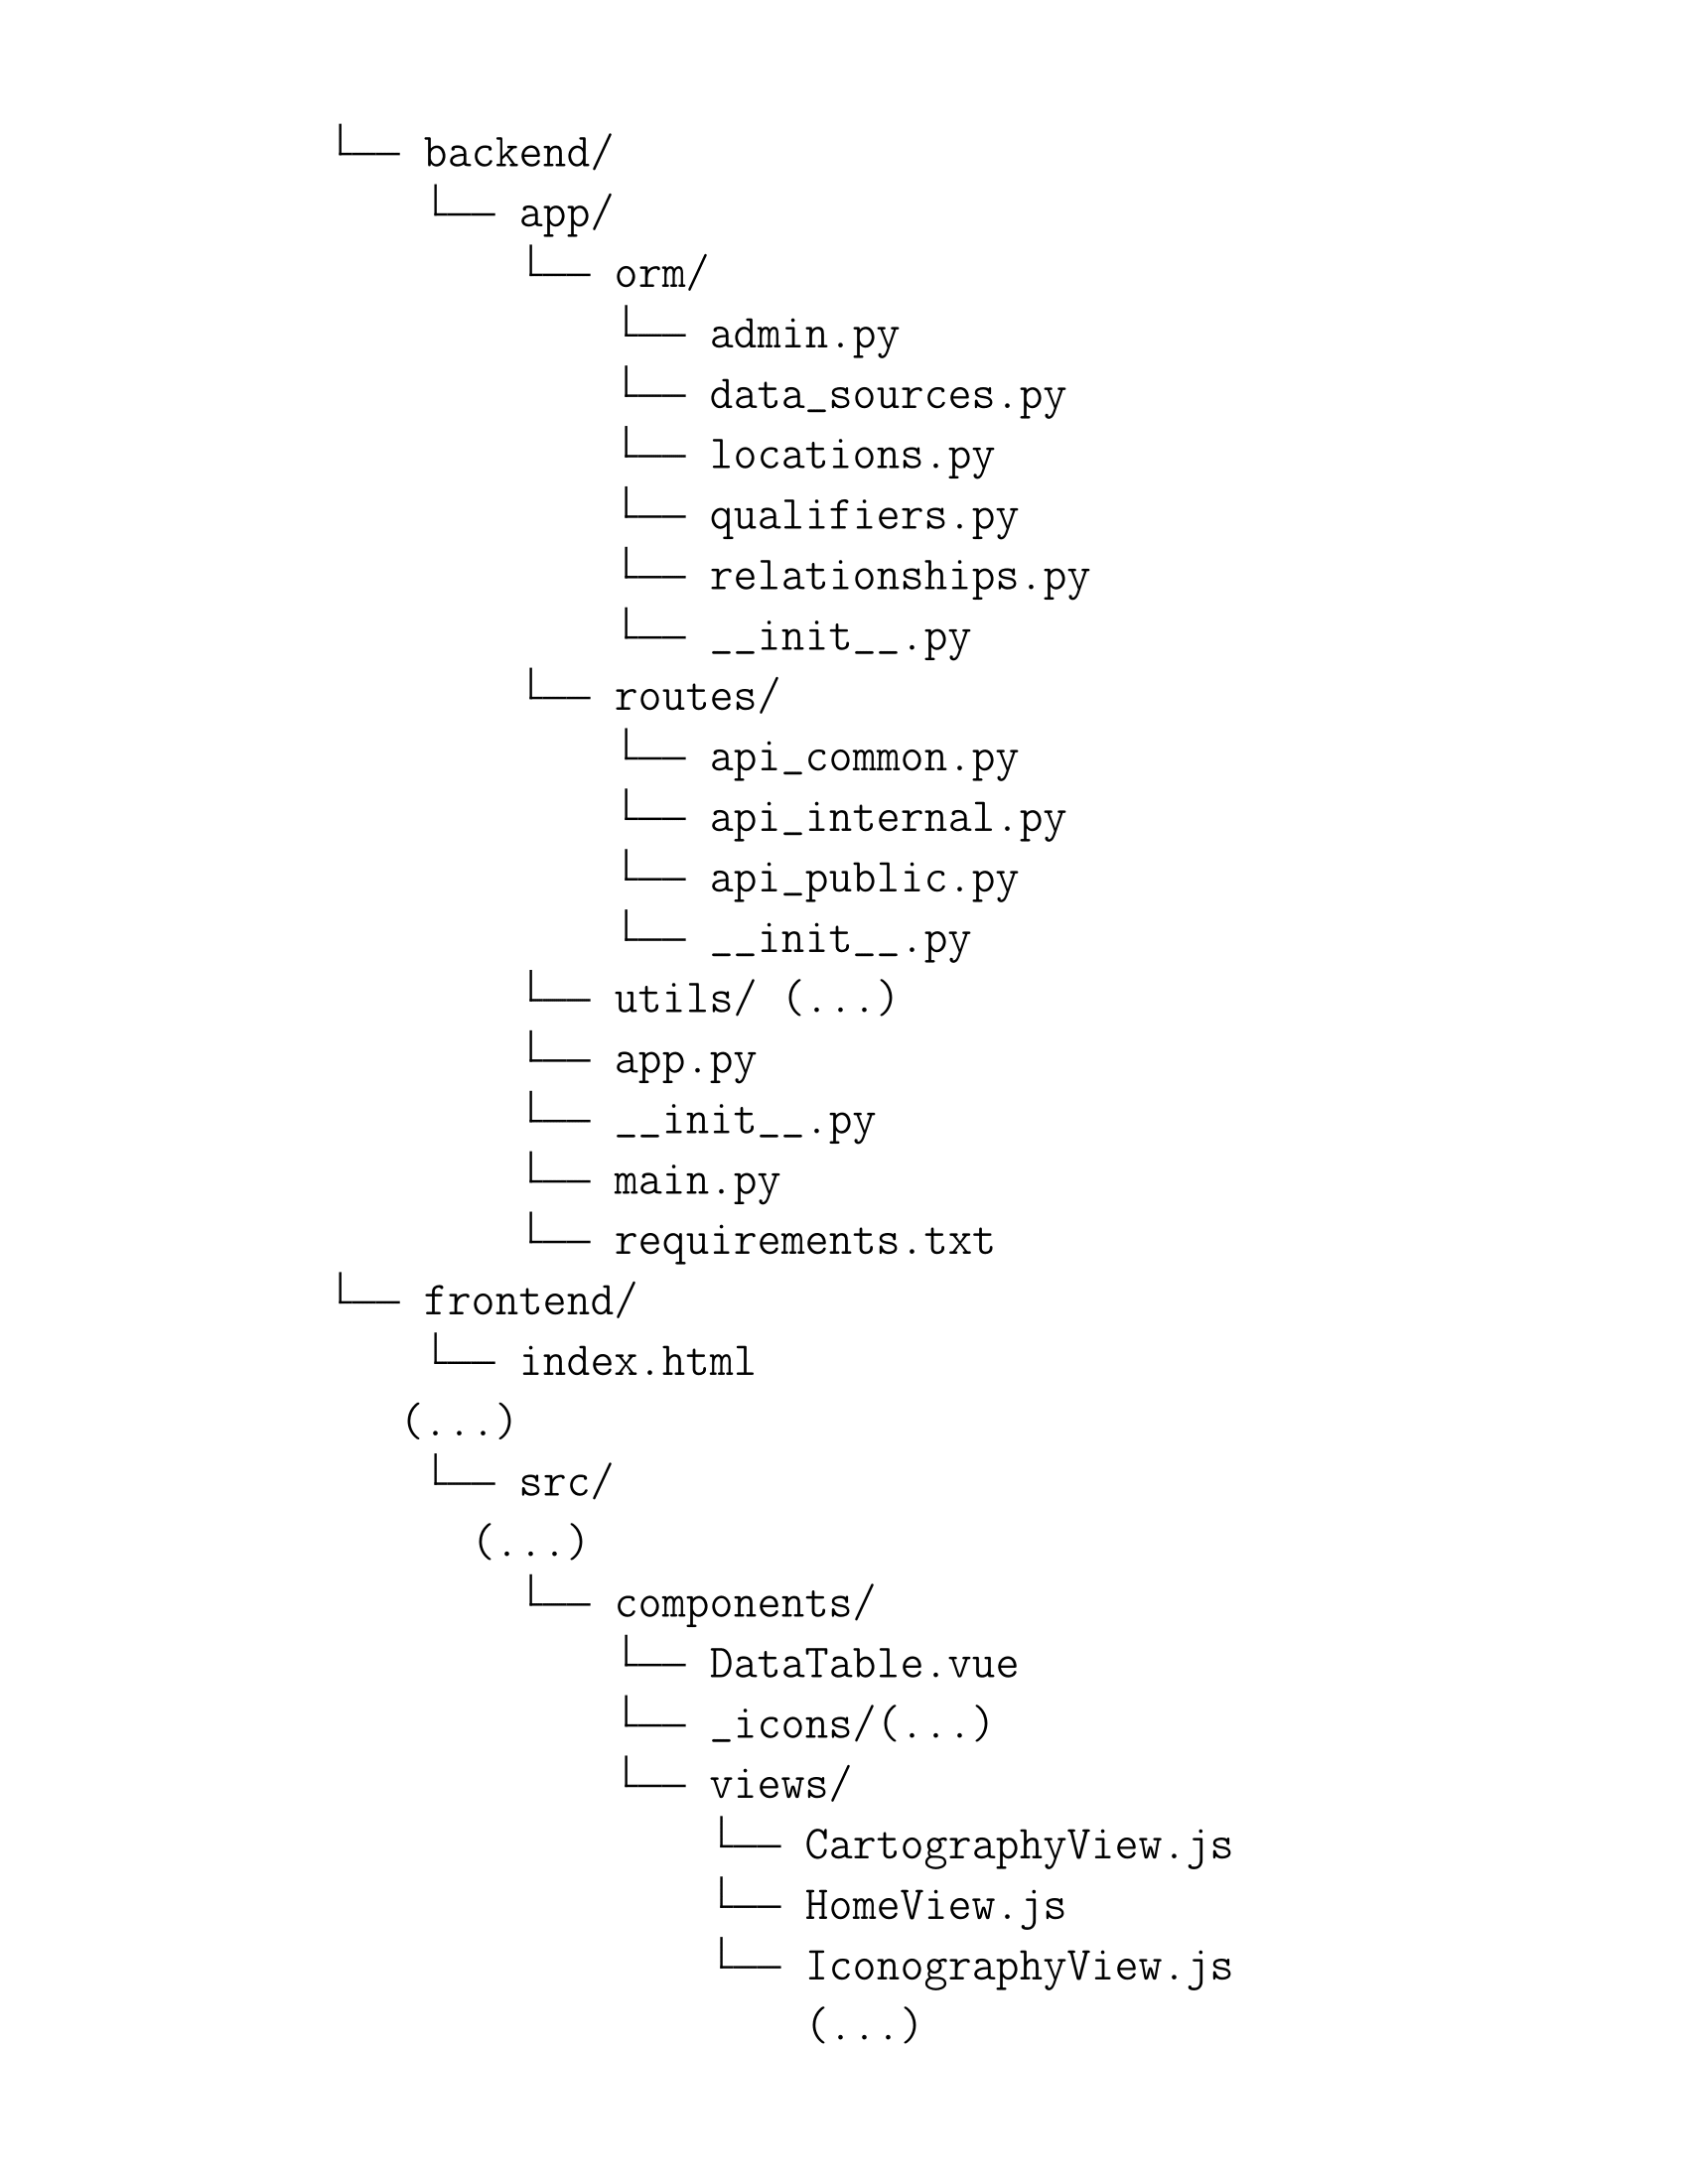
\includegraphics[width=0.5\linewidth]{images/architecture_appli_simplE.png}
    \caption{Arborescence simplifiée de l'application, \mhd.}
    \label{fig:app}
\end{figure}

\subsubsection{Quelques contraintes de développement}
Bien que le cadre de travail pour le développement de l'application intègre des outils puissants, leur prise en main peut être complexe pour un débutant. Chacun de ces outils peut sembler facile à utiliser individuellement, mais les combiner pour créer une architecture solide nécessite un certain temps d'adaptation. Par exemple, Vue.js offre de nombreux atouts de développement que nous avons présentés mais pour pouvoir l'utiliser, cela présuppose une solide maîtrise des langages du \textit{front-end} (\acrshort{html}, \acrshort{css} et JavaScript) -- ce qui n'est pas nécessairement le cas pour un stagiaire. Pourtant une compréhension approfondie de leur fonctionnement est indispensable pour exploiter pleinement les fonctionnalités de Vue.js. C'est pourquoi, après plusieurs tentatives et nombreux blocages, il a été décidé de développer la cartographie Web en dehors du \textit{Framework} Vue.js. Cette décision n'a pas d'impacts importants sur le développement général de l'application. 

\subsection{Les différents niveaux de communication client-serveur.}
\begin{figure}
    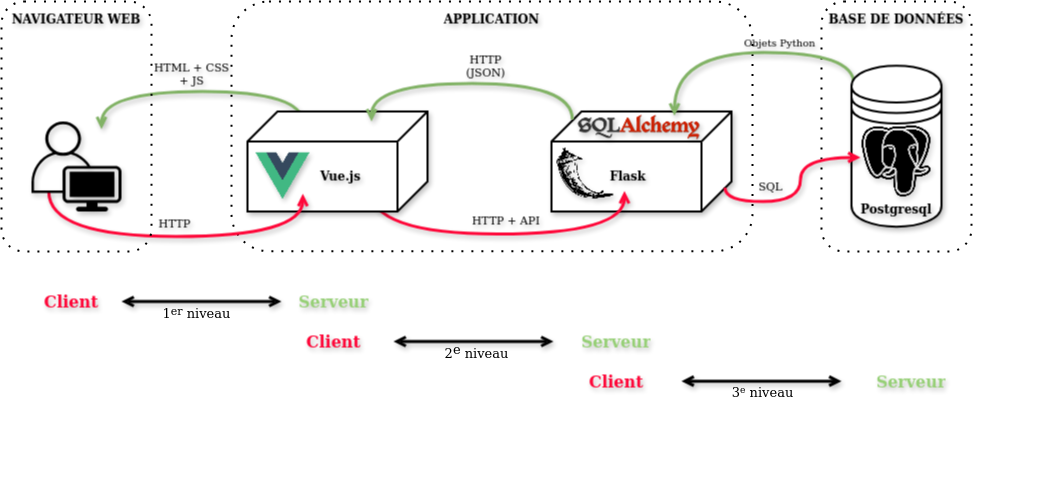
\includegraphics[width=1\linewidth]{images/Niveaux_communication_application.png}
    \caption{La communication client-serveur de l'application, \mhd.}
    \label{fig:enter-label}
\end{figure}
Pour transmettre l'information depuis la base de données jusqu'au navigateur Web via l'application, différents niveaux de communication client-serveur sont mis en place. Le premier niveau comprend le navigateur web, utilisé par l'utilisateur final, interagit avec l'application web construite avec Vue.js. Dans ce contexte, le navigateur agit en tant que client, envoyant des requêtes utilisateur à Vue.js, qui fonctionne comme un serveur pour ces interactions. Le deuxième niveau d'interaction, depuis Vue.js, après avoir traité l'interaction utilisateur, devient à son tour le client en envoyant des requêtes \acrshort{http} au back-end géré par Flask. Flask agit ici comme le serveur, répondant aux requêtes en fournissant les données nécessaires pour mettre à jour l'interface utilisateur. Le troisième, Flask, après avoir reçu la requête de Vue.js, se transforme en client en interrogeant la base de données PostgreSQL pour obtenir les informations demandées. SQLAlchemy joue un rôle intermédiaire ici, facilitant la communication entre Flask et PostgreSQL en convertissant les objets Python en requêtes SQL. PostgreSQL, en tant que serveur, répond à ces requêtes \acrshort{sql} en renvoyant les données nécessaires. À chaque étape, les rôles de client et serveur changent, illustrant la complexité et la modularité de l'architecture. Cette structure permet de découpler les différentes responsabilités de l'application, facilitant ainsi sa maintenance, son évolution et sa scalabilité. 
Pour un développement de l'application en local, l'architecture reste la même. 

%%%%%%%%%%%%%%%%%%%%%%%%%%%%%%%%%%%%%
\subsubsection{Conclusion du chapitre} 
En conclusion, les états successifs de la donnée du projet Richelieu illustrent la complexité croissante des objets numériques dans un environnement de plus en plus interconnecté. La structuration des données pour la cartographie Web démontre que la simple numérisation d’un corpus, qu’il soit iconographique ou cartographique, dépasse largement la production d’une image numérique. Il s'agit de la création d’un objet numérique sophistiqué, enrichi de métadonnées descriptives et structurelles, qui permet de révéler la profondeur et la richesse de l’information contenue dans ces documents. Cela amène à s'interroger sur le passage du Web de documents, où les ressources sont principalement statiques, au Web de données, où l'information est dynamique, interrogeable et exploitable, créant ainsi de nouvelles perspectives pour la recherche et la diffusion du savoir.

%%%%%%%%%%%%%%%%%%%%%%%%%%%%%%%%%%%%%
\subsubsection{Conclusion de la première partie} 
La base de données du projet Richelieu, bien que peu volumineuse avec ses 100~000 entrées, reflète avec précision les multiples facettes du quartier et incarne l'essence même de son nom : Richelieu, un lieu riche en histoire et en significations. Ce lieu occupe une position centrale dans la conception et l'orientation du projet. Le système développé pour soutenir cette ambition est à la fois robuste et d'une complexité technique relative, nécessitant un véritable investissement en temps pour être analysé, compris et maîtrisé par l'ingénieure novice. Après de longues étapes de saisie, d'encodage et de stockage des données, le projet s’est doté de l’infrastructure technique nécessaire pour réaliser ses ambitions scientifiques et mettre en lumière la richesse des informations qu’il contient.